\chapter{Proposta}\label{cap4}

\section{Usuários}


\section{Terminologias Existentes}

\subsection{Tesauros}

\subsection{Ontologias Existente}


\section{Descrição do Ambiente Web}
Audiobook, basicamente são livros narrados. Ou seja, são gravações dos conteúdos de livros, cujo o mesmo é lido. Estes audiobook posuem diversos formatos informacionais, como MP3 e WMA, entre outro, podendo ser pagos ou gratuitos, dependendo da plataforma à qual os audibooks, encontram-se disponíveis.
Ideal para os leitores que gostam de praticar o habito da leitura, porém não dispõem o tempo necessário para exercer esta atividade. Estes audiobooks, podem possuir diversas funcionalidade que enriquecem a esculta, como efeitos sonoros, variações no tom de voz, entre outros meios que evitam a ociosidade na esculta.
Possuem uma quantidade de exemplares no idioma português relativamente baixa, porém possuem uma grande variedade de conteúdo internacional, principalmente no idioma inglês, um dos maiores mercados de audiobooks disponível.

\section{Cronograma}
A criação das atividades desse cronograma foram baseadas no plano de ensino da disciplina Tópicos especiais em Engenharia de Software. Este plano foi desenvolvido para o primeiro semestre letivo no ano de 2015.

 \begin{figure}[ht]
  \centering
    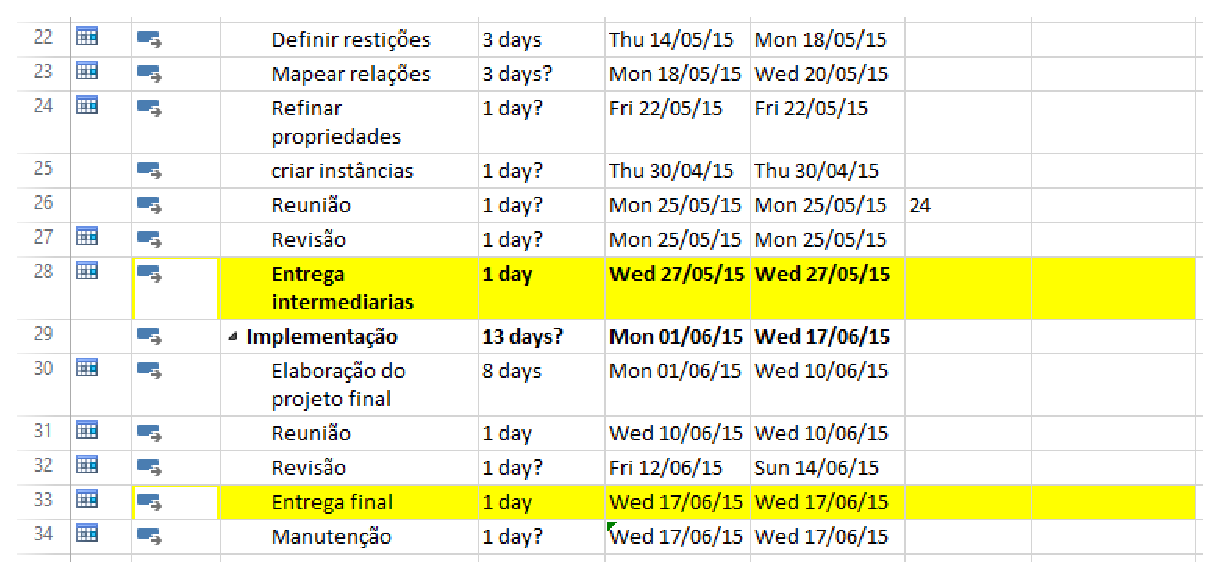
\includegraphics[keepaspectratio=true,scale=0.5]{figuras/cronograma.eps}
  \caption{Cronograma do projeto}
\end{figure}